\section{Manejo de Figuras: Tablas, Gráficos e Imágenes}
\LaTeX ofrece potentes herramientas para incluir y formatear figuras, tablas e imágenes con precisión tipográfica. 

\subsection{Manejo de Tablas}
\LaTeX{} ofrece control preciso sobre tablas mediante entornos \texttt{tabular} y \texttt{table} \cite{latex_project}. La principal diferencia entre ambos es que \texttt{tabular} se usa para crear la estructura de la tabla, mientras que \texttt{table} es un entorno flotante que permite agregar títulos, etiquetas y controlar la posición de la tabla en el documento.

\subsubsection{Tabla Básica: Entorno tabular}

En su forma más simple, el entorno \texttt{tabular} se utiliza para crear tablas sin título ni numeración, como se muestra en el siguiente ejemplo:

\begin{tabular}{|l|c|r|}   
\hline 
\textbf{Nombre} & \textbf{Edad} & \textbf{Ciudad} \\
\hline
Juan Pérez & 25 & San José \\
María Gómez & 30 & Alajuela \\
\hline
\end{tabular}

Para crear esta tabla, se utiliza el siguiente código:

\begin{verbatim}
\begin{tabular}{|l|c|r|}
\hline
\textbf{Nombre} & \textbf{Edad} & \textbf{Ciudad} \\
\hline
Juan Pérez & 25 & San José \\
María Gómez & 30 & Alajuela \\
\hline
\end{tabular}
\end{verbatim}

\subsubsection{Tabla Flotante Completa}

Como se mencionó anteriormente, la tabla tabular no permite agregar títulos ni etiquetas para referencias cruzadas. Para esto, se utiliza el entorno \texttt{table}, que es un entorno flotante \cite{latex_project}. Esto significa que \LaTeX puede mover la tabla a una posición óptima en el documento, como la parte superior o inferior de una página.

\begin{table}[h]
\centering
\caption{Ejemplo de tabla flotante}
\label{tab:tabla_ejemplo}
\begin{tabular}{lccc}
\toprule
\textbf{Nombre} & \textbf{Edad} & \textbf{Ciudad} \\
\midrule
Juan Pérez & 25 & San José \\
María Gómez & 30 & Alajuela \\
\bottomrule
\end{tabular}
\end{table}

El siguiente código muestra cómo crear una tabla flotante con título y etiqueta, tal como se observa en el Cuadro \ref{tab:tabla_ejemplo}:

\begin{verbatim}
\begin{table}[h] % h=here, t=top, b=bottom
\centering
\caption{Ejemplo de tabla flotante}
\label{tab:tabla_ejemplo}
\begin{tabular}{lccc}
\toprule
\textbf{Nombre} & \textbf{Edad} & 
\textbf{Ciudad} \\
\midrule
Juan Pérez & 25 & San José \\
María Gómez & 30 & Alajuela \\
\bottomrule
\end{tabular}
\end{table}
\end{verbatim}

Para definir la posición de un elemento flotante, se utilizan las opciones \texttt{h} (here), \texttt{t} (top), \texttt{b} (bottom) y \texttt{p} (page of floats). Por ejemplo, \texttt{[ht]} indica que \LaTeX intentará colocar la tabla aquí o en la parte superior de la página.

\subsection{Manejo de Gráficos e Imágenes}

Para incluir gráficos e imágenes, se utiliza el paquete \texttt{graphicx} \cite{graphicx}. Este paquete permite insertar imágenes en formatos comunes como PNG, JPEG y PDF, y ofrece opciones para escalar, rotar y recortar las imágenes.

\subsubsection{Figuras Individuales}

La siguiente figura muestra un ejemplo de cómo incluir una imagen utilizando el paquete \texttt{graphicx}:

\begin{figure}[h]
\centering
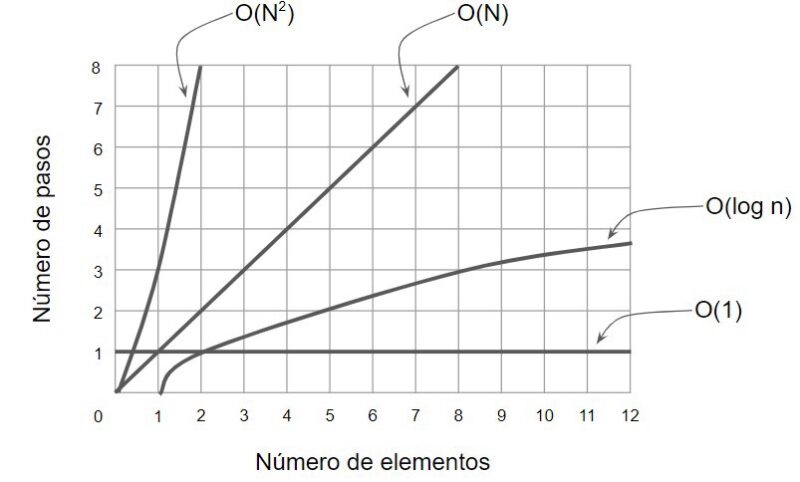
\includegraphics[width=0.45\textwidth]{ejemplo_imagen.jpg}
\caption{Ejemplo de imagen.}
\label{fig:ejemplo_imagen}
\end{figure}

Para insertar la Figura \ref{fig:ejemplo_imagen}, se utiliza el siguiente código:

\begin{verbatim}
\usepackage{graphicx}     % Paquete esencial
\begin{figure}[h]
\centering
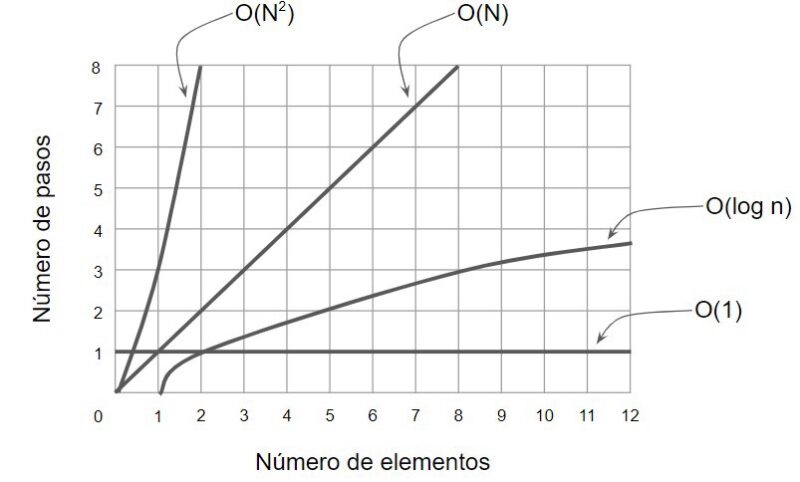
\includegraphics[width=0.45\textwidth]
{ejemplo_imagen.jpg}
\caption{Ejemplo de imagen}
\label{fig:ejemplo_imagen}
\end{figure}
\end{verbatim}

La Figura \ref{fig:ejemplo_imagen} se escaló al 45\% del ancho del texto, pero también se pueden usar otras opciones como \texttt{height} para establecer una altura fija o \texttt{scale} para escalar proporcionalmente.

\begin{verbatim}
\includegraphics[height=5cm]{fig}
\includegraphics[scale=0.5]{fig}
\end{verbatim}

\subsubsection{Subfiguras Múltiples}

A través del paquete \texttt{subcaption} \cite{subcaption}, es posible incluir varias subfiguras dentro de una figura principal, cada una con su propio título y etiqueta. Esto es útil para comparar diferentes configuraciones o resultados en un mismo bloque visual.

\begin{figure}[ht]
\centering
\begin{subfigure}{0.4\textwidth}
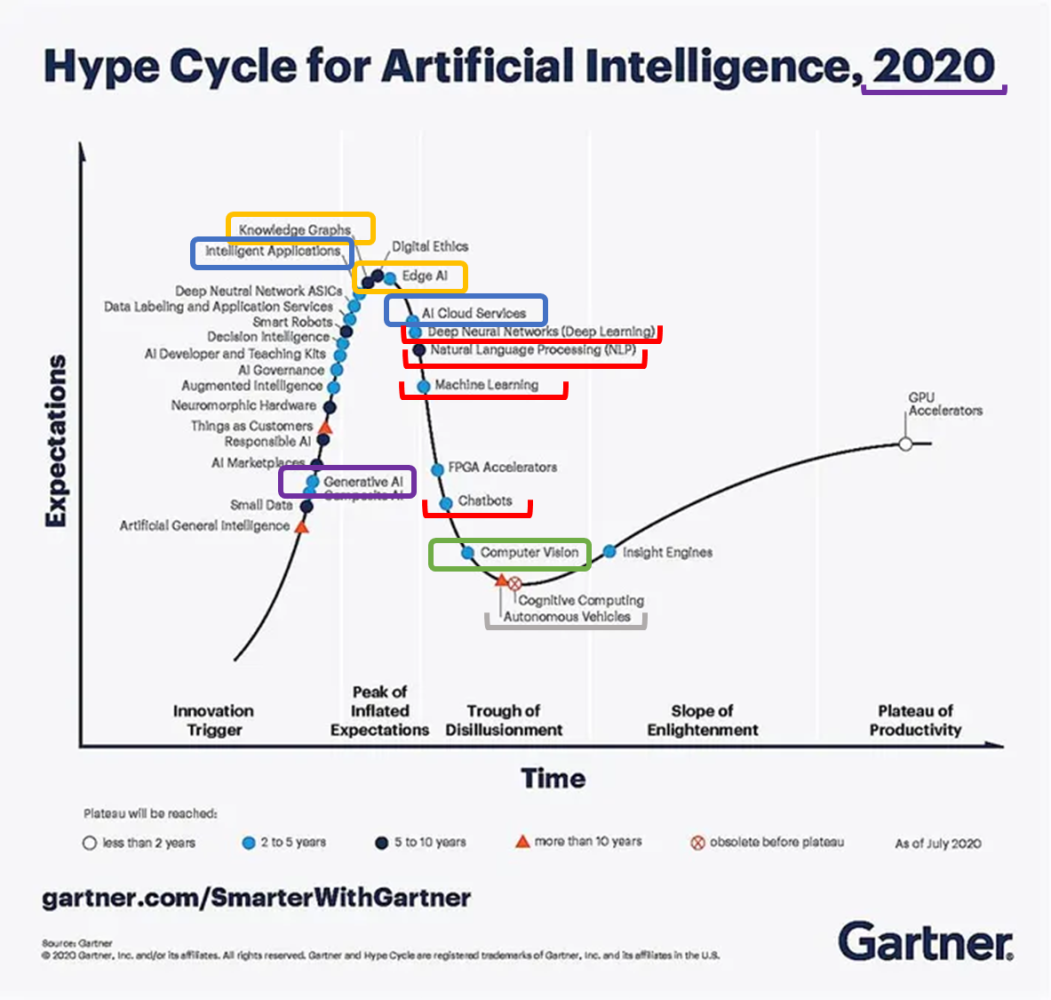
\includegraphics[width=\textwidth]{ia_2020.png}
\caption{IA en 2020}
\label{fig:ia_2020}
\end{subfigure}
\hfill
\begin{subfigure}{0.4\textwidth}
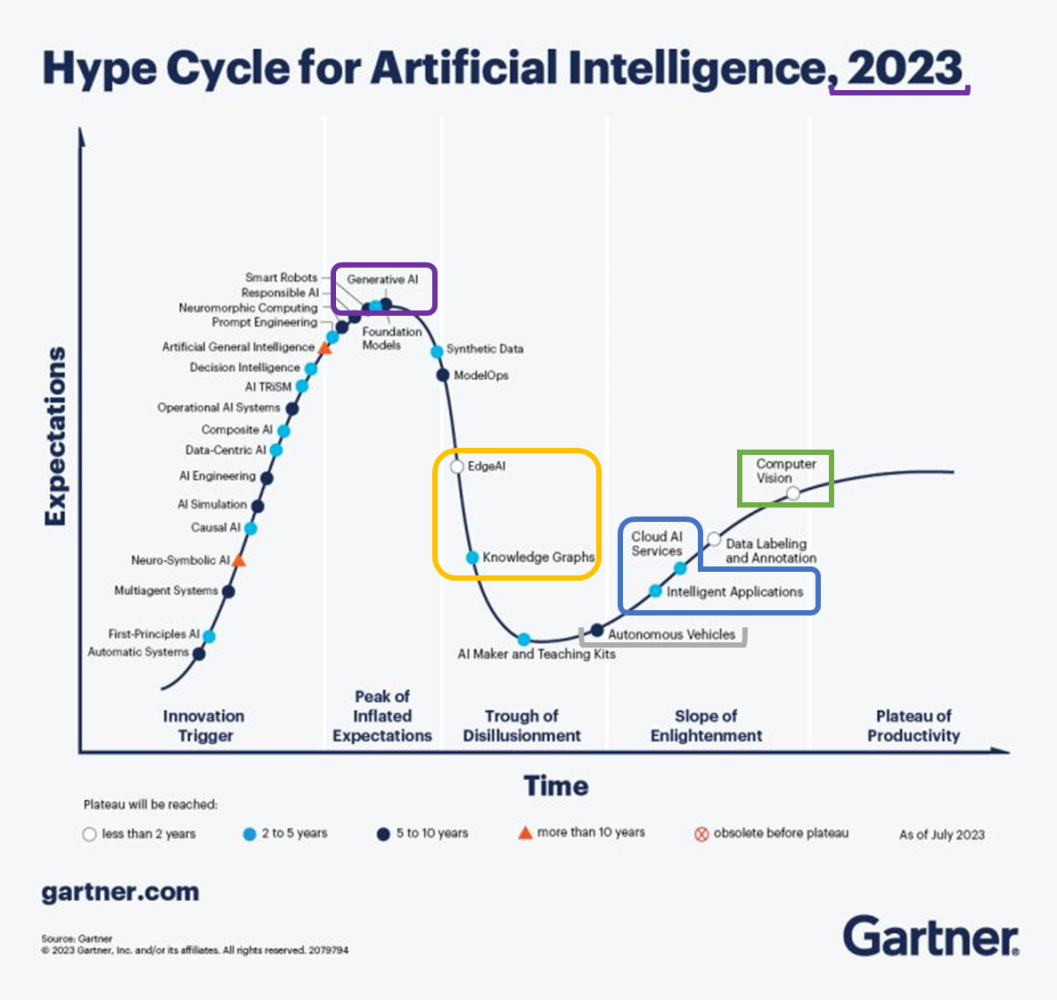
\includegraphics[width=\textwidth]{ia_2023.png}
\caption{IA en 2023}
\label{fig:ia_2023}
\end{subfigure}
\caption{Comparativa de proyecciones de IA.}
\label{fig:comparativa_ia}
\end{figure}


Para incluir la Figura \ref{fig:comparativa_ia} con subfiguras, se utiliza el siguiente código:


\begin{verbatim}
\usepackage{subcaption}
\begin{figure}[ht]
\centering
\begin{subfigure}{0.4\textwidth}
\includegraphics[width=\textwidth]{fig1}
\caption{IA en 2020}
\label{fig:ia_2020}
\end{subfigure}
\hfill
\begin{subfigure}{0.4\textwidth}
\includegraphics[width=\textwidth]{fig2}
\caption{IA en 2023}
\label{fig:ia_2023}
\end{subfigure}
\caption{Comparativa de proyecciones de IA.}
\label{fig:comparativa_ia}
\end{figure}
\end{verbatim}

\subsubsection{Gráficos con TikZ (Vectoriales)}

Una de las principales fortalezas de \LaTeX{} es la capacidad de crear gráficos vectoriales directamente en el documento utilizando el paquete \texttt{tikz} \cite{tikz_manual}. Esto permite generar gráficos de alta calidad que se escalan sin pérdida de resolución, ideales para diagramas, funciones matemáticas y visualizaciones personalizadas:

\begin{figure}[h]
\centering
\begin{tikzpicture}
\draw[thick,->] (0,0) -- (7,0) node[right]{$x$};
\draw[thick,->] (0,-3) -- (0,3) node[above]{$y$};
\draw[domain=0:7,smooth,blue,thick] 
    plot (\x, {sin(\x r)*1.5});
\node at (2,1.8) {$\sin(x)$};
\end{tikzpicture}
\caption{Función seno generada con TikZ.}
\label{fig:tikz}
\end{figure}

La función seno en la Figura \ref{fig:tikz} se creó con el siguiente código:

\begin{verbatim}
\usepackage{tikz}
\begin{figure}[h]
\centering
\begin{tikzpicture}
\draw[thick,->] (0,0)--(7,0) node[right]{$x$};
\draw[thick,->] (0,-3)--(0,3) node[above]{$y$};
\draw[domain=0:7,smooth,blue,thick] 
    plot (\x, {sin(\x r)*1.5});
\node at (2,1.8) {$\sin(x)$};
\end{tikzpicture}
\caption{Función seno generada con TikZ.}
\label{fig:tikz}
\end{figure}
\end{verbatim}

\subsection{Figuras y Tablas Lado a Lado: minipage}

El entorno \texttt{minipage} permite combinar figuras y tablas en una sola unidad visual \cite{latex_project}.

\begin{figure}[ht]
\begin{minipage}{0.15\textwidth}
\centering
\begin{tikzpicture}[scale=0.4]
\draw[thick,->](0,0)--(14,0) node[right]{t};
\draw[thick,->](0,-3)--(0,5) node[above]{V};
\draw[domain=0:4,smooth,green,thick] plot (\x, {\x});
\draw[domain=4:6,smooth,blue,thick] plot (\x, {4});
\draw[domain=6:9,smooth,red,thick] plot (\x, {16-2*\x});
\draw[domain=9:10,smooth,blue,thick] plot (\x, {-2});
\draw[domain=10:12,smooth,green,thick] plot (\x, {\x-12});
\end{tikzpicture}
\caption*{Gráfico}
\end{minipage}
\hfill
\begin{minipage}{0.15\textwidth}
\centering
\footnotesize
\begin{tabular}{lcc}
\toprule
\textbf{Tiempo} & \textbf{Velocidad} \\
\midrule
4s & 4m/s \\
6s & 4m/s \\
8s & 0m/s \\
9s & -2m/s \\
10s & -2m/s \\
12s & 0m/s \\
\bottomrule
\end{tabular}
\caption*{Datos}
\end{minipage}
\caption{Observación de gráfico y tabla lado a lado.}
\label{fig:ejemplo_minipage}
\end{figure}

La Figura \ref{fig:ejemplo_minipage} se creó con el siguiente código:

\begin{verbatim}
\begin{figure}[ht]
\begin{minipage}{0.15\textwidth}
\centering
\begin{tikzpicture}[scale=0.4]
\draw[thick,->](0,0)--(14,0) node[right]{t};
\draw[thick,->](0,-3)--(0,5) node[above]{V};
\draw[domain=0:4,smooth,green,thick] 
plot (\x, {\x});
\draw[domain=4:6,smooth,blue,thick] 
plot (\x, {4});
\draw[domain=6:9,smooth,red,thick] 
plot (\x, {16-2*\x});
\draw[domain=9:10,smooth,blue,thick] 
plot (\x, {-2});
\draw[domain=10:12,smooth,green,thick] 
plot (\x, {\x-12});
\end{tikzpicture}
\caption*{Gráfico}
\end{minipage}
\hfill
\begin{minipage}{0.15\textwidth}
\centering
\footnotesize
\begin{tabular}{lcc}
\toprule
\textbf{Tiempo} & \textbf{Velocidad} \\
\midrule
4s & 4m/s \\
6s & 4m/s \\
8s & 0m/s \\
9s & -2m/s \\
10s & -2m/s \\
12s & 0m/s \\
\bottomrule
\end{tabular}
\caption*{Datos}
\end{minipage}
\caption{Observación de gráfico y 
tabla lado a lado.}
\label{fig:ejemplo_minipage}
\end{figure}
\end{verbatim}
